\subsection{Beta-only useful delivery and complete profit}
Competent Beta includes the current frontier workflow, ordinary tools, existing equivalents and useful source-agent local artifacts. It requires no newly admitted graph skill and no optional capability campaign. The following commercial results stand independently of the optional Alpha findings.
\begin{table}[htbp]\centering\small\begin{tabular}{lrrrrr}
\toprule
Condition & Useful jobs & Human ref.* & Charge* & Cost/useful & Net profit\\\midrule
Conservative & 4.2 & \usd{15,228} & \usd{4,639} & \usd{5,405} & \usd{-3,976}\\
Central & 54.7 & \usd{26,952} & \usd{10,870} & \usd{1,020} & \usd{522,787}\\
Favorable & 150.2 & \usd{43,875} & \usd{24,034} & \usd{1,059} & \usd{3,421,787}\\
\bottomrule\end{tabular}\caption{Beta-only commercial core. Project counts and complete profit are enterprise means. *Human reference and gross charge use the same truly useful, collected cohort, including richer scopes. Complete cost pools all paid and failed work, overhead, setup and discovery over all truly accepted outcomes, including valid outcomes whose payment was not authorized. The columns are not an algebraic per-job profit calculation. USD; simulated.}\end{table}
\begin{table}[htbp]\centering\small\begin{tabular}{lrrrrr}
\toprule
Condition & Collections & Refunds & All costs & Profit 5th & Profit 95th\\\midrule
Conservative & \usd{23,222} & \usd{4,378} & \usd{22,820} & \usd{-19,238} & \usd{15,082}\\
Central & \usd{609,327} & \usd{30,748} & \usd{55,792} & \usd{225,770} & \usd{951,875}\\
Favorable & \usd{3,616,321} & \usd{35,451} & \usd{159,083} & \usd{2,109,877} & \usd{5,157,358}\\
\bottomrule\end{tabular}\caption{Mean settled gross receipts, paid refunds and complete costs; profit distribution across all worlds. Fees are already in costs. Unpaid refund liabilities also reduce profit. Seed capital is not revenue.}\end{table}

\textbf{Conservative.} Beta delivered 4.2 truly useful projects (0.18 per operating month), of which 3.8 were useful and collected. The gross charge in that paid cohort averaged \usd{4,639}; its matched human reference averaged \usd{15,228}. Their arithmetic reference-price difference was \usd{10,589}, or a mean 69.5\% discount across those projects. This is not observed buyer savings or proof that every buyer would otherwise purchase the human service. The mean monthly posted base-scope price was \usd{4,237} (32.6\% of the base reference), distinct from the sold scope mix. The modeled purchase share was 25.9\% across 24.4 qualified opportunities. Profit was positive in 31.0\% of simulated worlds; cash-shortfall shutdown occurred in 2.4\%. These are scenario frequencies, not calibrated real-world success probabilities.

\textbf{Central.} Beta delivered 54.7 truly useful projects (2.28 per operating month), of which 52.5 were useful and collected. The gross charge in that paid cohort averaged \usd{10,870}; its matched human reference averaged \usd{26,952}. Their arithmetic reference-price difference was \usd{16,083}, or a mean 59.7\% discount across those projects. This is not observed buyer savings or proof that every buyer would otherwise purchase the human service. The mean monthly posted base-scope price was \usd{9,353} (40.9\% of the base reference), distinct from the sold scope mix. The modeled purchase share was 58.6\% across 109.2 qualified opportunities. Profit was positive in 100.0\% of simulated worlds; cash-shortfall shutdown occurred in 0.0\%. These are scenario frequencies, not calibrated real-world success probabilities.

\textbf{Favorable.} Beta delivered 150.2 truly useful projects (6.26 per operating month), of which 148.6 were useful and collected. The gross charge in that paid cohort averaged \usd{24,034}; its matched human reference averaged \usd{43,875}. Their arithmetic reference-price difference was \usd{19,841}, or a mean 45.2\% discount across those projects. This is not observed buyer savings or proof that every buyer would otherwise purchase the human service. The mean monthly posted base-scope price was \usd{20,337} (54.7\% of the base reference), distinct from the sold scope mix. The modeled purchase share was 66.7\% across 245.7 qualified opportunities. Profit was positive in 100.0\% of simulated worlds; cash-shortfall shutdown occurred in 0.0\%. These are scenario frequencies, not calibrated real-world success probabilities.

\textbf{Quality is a separate condition.} Material errors among approved Beta deliveries were 23.5\%, 6.3\% and 1.3\% in conservative, central and favorable conditions. Removing all otherwise undetected paid false-pass receipts as a terminal valuation stress leaves central profit of \usd{515,390} and favorable profit of \usd{3,411,472}. This supports the modeled useful-work margin without treating erroneous receipts as indispensable. It does not create a new refund-timing trajectory, establish a full liability ceiling, or prove that buyers accept the residual error rate. A required error budget tighter than a scenario's residual rate would require a stronger validator or narrower offering.

\subsection{Available surplus, seed and throughput}
\begin{table}[htbp]\centering\scriptsize\begin{tabular}{lrrrrr}
\toprule
Condition & Cash, m24 & Reserve, m24 & Receivable, m24 & Excess*, m24 & Excess*, m27\\\midrule
Conservative & \usd{14,946} & \usd{2,166} & \usd{1,726} & \usd{1,766} & \usd{2,412}\\
Central & \usd{519,077} & \usd{9,243} & \usd{27,260} & \usd{489,833} & \usd{516,107}\\
Favorable & \usd{3,260,307} & \usd{38,830} & \usd{190,726} & \usd{3,201,477} & \usd{3,386,459}\\
\bottomrule\end{tabular}\caption{Beta cash stocks, USD means. *Nonnegative cash available after protecting known obligations, the declared reserve and the entire original USD20,000 seed. Receivables cannot fund current spending. Known refunds/recovery are not subtracted twice when already inside reserve. The settled endpoint retains the operating reserve policy; it is not liquidation value. Nonnegative world-level stocks are averaged, so a positive mean excess does not negate conservative losses.}\end{table}
Central month-24 uncommitted cash was \usd{509,833}, including possible seed, while \usd{489,833} remained after preserving the entire seed. Its 5th--95th percentile range above seed was \usd{209,585} to \usd{883,502}. The conservative median excess above seed was zero even though many enterprises retained some original capital. These stocks differ from accrual-like complete profit and are never summed across months.
The primary runs show no capacity-deferred orders. Their achieved throughput therefore demonstrates conditional operation at the tested demand, not a measured saturation point or an Alpha-driven capacity expansion. The resource screens and scale stresses locate conditional bottlenecks; actual provider quotas, latency and validator capacity require later measurement. Increased volume by itself is not self-acceleration.
\begin{figure}[htbp]\centering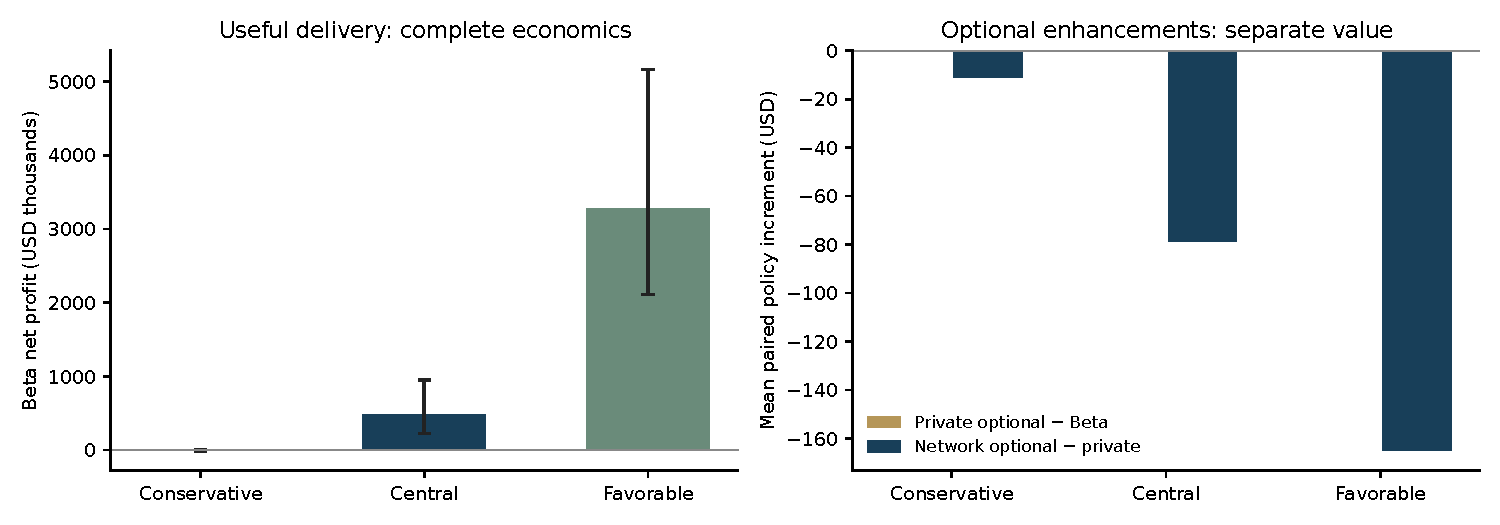
\includegraphics[width=\linewidth]{generated/results_overview.pdf}\caption{Commercial core first. Left: Beta complete-profit medians and 5th--95th percentile ranges. Right: paired mean policy increments from optional private capability decisions and network availability. The scales differ deliberately: large service economics and small enhancement effects are distinct questions.}\end{figure}
\subsection{Optional retained Alpha, sharing and investment}
\begin{table}[htbp]\centering\small\begin{tabular}{lrrrrr}
\toprule
Condition & Network $-$ Beta & Network $-$ private & Retain & Admit & Feedback\\\midrule
Conservative & \usd{-11} & \usd{-11} & 0.0\% & 0.00 & 0.0\%\\
Central & \usd{-79} & \usd{-79} & 0.0\% & 0.00 & 0.0\%\\
Favorable & \usd{-165} & \usd{-165} & 0.0\% & 0.00 & 0.0\%\\
\bottomrule\end{tabular}\caption{Optional-policy mean increments and all-world frequencies, kept separate from Beta commercial success. Retain is an additional B-package purchase. Feedback requires an operating-funded package linking useful collected source work to useful fresh recipient work, positive total and quality-adjusted paired value, and no separate C construction campaign. It is descriptive, not a mandatory investment count.}\end{table}
No primary world purchased portable retention or optional separate capability construction. Ordinary source-agent artifacts remain available under Beta; paid candidate scans and nominated candidates do not establish additional Alpha. The tested policy declined the incremental expenditures. Its small negative network effects reflect the cost and incidental resource consequences of searching, not destruction of the profitable commercial core. This is evidence of the tested policy choosing restraint, not proof that every possible retained capability is worthless or that global optimality has been established.

Conservative: network availability changed mean profit by \usd{-11} (Monte Carlo standard error \usd{0.41}; 5th--95th percentile \usd{-27} to \usd{0}). Private optional decisions changed profit by \usd{0}. Paid scans averaged 1.9, nominated candidates 0.3, and upfront B purchases \usd{0}. There were 0.00 useful capability--project reuse pairs; separate capsules can create multiple pairs for one project. The paired policy effect on distinct useful projects was 0.00. Endogenous network pricing changed mean profit by \usd{8,404} relative to the fixed 65\% diagnostic; this comparison includes any induced resource decisions.

Central: network availability changed mean profit by \usd{-79} (Monte Carlo standard error \usd{1.60}; 5th--95th percentile \usd{-148} to \usd{-31}). Private optional decisions changed profit by \usd{0}. Paid scans averaged 20.4, nominated candidates 2.0, and upfront B purchases \usd{0}. There were 0.00 useful capability--project reuse pairs; separate capsules can create multiple pairs for one project. The paired policy effect on distinct useful projects was 0.00. Endogenous network pricing changed mean profit by \usd{161,153} relative to the fixed 65\% diagnostic; this comparison includes any induced resource decisions.

Favorable: network availability changed mean profit by \usd{-165} (Monte Carlo standard error \usd{2.13}; 5th--95th percentile \usd{-250} to \usd{-94}). Private optional decisions changed profit by \usd{0}. Paid scans averaged 53.3, nominated candidates 3.0, and upfront B purchases \usd{0}. There were 0.00 useful capability--project reuse pairs; separate capsules can create multiple pairs for one project. The paired policy effect on distinct useful projects was 0.00. Endogenous network pricing changed mean profit by \usd{176,018} relative to the fixed 65\% diagnostic; this comparison includes any induced resource decisions.
\begin{table}[htbp]\centering\small\begin{tabular}{lrrrrr}
\toprule
Condition & Beta A & Beta B & Beta C* & Network B & Later C\\\midrule
Conservative & \usd{17,569} & \usd{0} & \usd{5,251} & \usd{11} & \usd{0}\\
Central & \usd{50,541} & \usd{0} & \usd{5,251} & \usd{79} & \usd{0}\\
Favorable & \usd{153,833} & \usd{0} & \usd{5,251} & \usd{165} & \usd{0}\\
\bottomrule\end{tabular}\caption{Disjoint complete-cost records, USD means. A includes delivery, within-job learning, qualification, fees and allocated overhead. B includes extra scans, failed candidates, retention and reuse. *C includes initial bounded venture discovery; later optional C campaigns are identified separately. Refunds reverse revenue, and no source-job construction is charged again to B.}\end{table}
The primary confirmation does not supply a population of funded admissions from which to estimate admission precision or realized skill repayment. Directed funded and recovery fixtures verify software/accounting branches only; their forced capital action is not economic-selection evidence. Any actual funded sensitivity path is separately labeled and retains its all-world frequency. Profitable delivery, useful retained Alpha, productive reinvestment and self-acceleration remain different claims.
